% This is my HW 6 solution set.

\documentclass[12pt, leqno]{article}
\usepackage{amsfonts, amsmath, amssymb}
\usepackage{fancyhdr}
\usepackage{hyperref}
\usepackage{graphicx}
\newcounter{qcounter}
\usepackage[lofdepth,lotdepth]{subfig}
\usepackage[maxfloats=40]{morefloats}
\usepackage{float}
\usepackage{}
\usepackage[english]{babel}
\usepackage{tabularx}
\providecommand{\abs}[1]{\lvert#1\rvert} % absolute value
\providecommand{\normd}{\mathcal{N}} % normal distribution
\providecommand{\norm}[1]{\lVert#1\rVert} % norm
\newcommand{\macheps}{\epsilon_{\mbox{\scriptsize mach}}}
\usepackage[ampersand]{easylist}
\makeatletter
\newcommand{\distas}[1]{\mathbin{\overset{#1}{\kern\z@\sim}}}%
\newsavebox{\mybox}\newsavebox{\mysim}
\newcommand{\distras}[1]{%
  \savebox{\mybox}{\hbox{\kern3pt$\scriptstyle#1$\kern3pt}}%
  \savebox{\mysim}{\hbox{$\sim$}}%
  \mathbin{\overset{#1}{\kern\z@\resizebox{\wd\mybox}{\ht\mysim}{$\sim$}}}%
}
\makeatother

\begin{document}
\pagestyle{fancy}
\lhead{Syed Rahman}
\rhead{STA6866}

\begin{center}
{\large {\bf Homework 7}} \\
\end{center}

\paragraph{1.} We consider the following hierarchical Bayes model:
\[
X_i|\theta_i \sim \normd (\theta_i,1)
\]
\[
\theta_i| \mu, \tau^2 \sim \normd (\mu,\tau^2)
\]
\[
\mu \sim \normd(0,1000)
\]
\[
\tau^2 \sim \chi^2_1
\]
where $\mu$ and $\tau$ are considered indenpendent.
We run a Gibbs-Sampler using $JAGS$ and generate $100,000$ samples
using a thin of 1 and a burn-in of 10,000. The posterior densities
were fit using the $density$ function in $R$. These are presented in Figures
\ref{dens1} and \ref{dens2}.
\begin{figure}
\begin{center}
  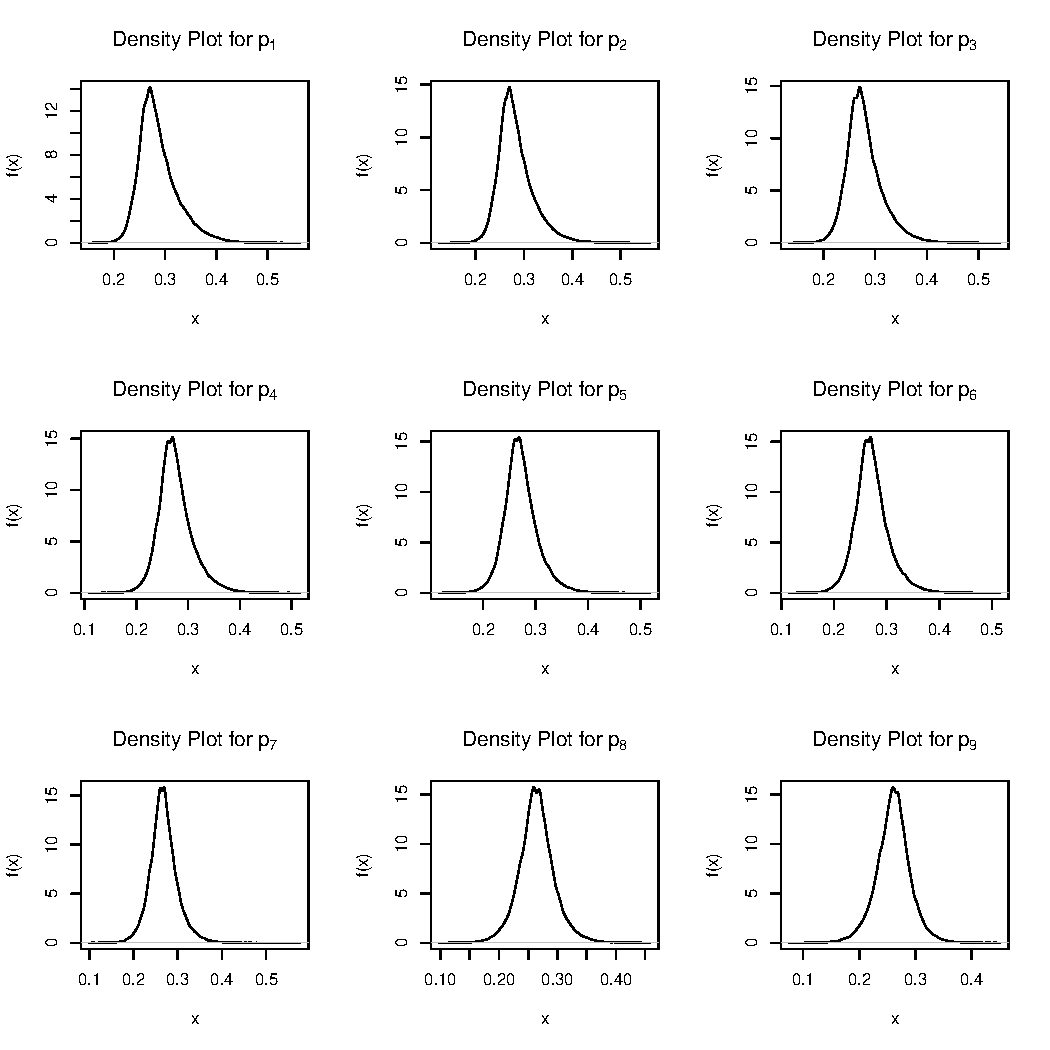
\includegraphics[scale=0.8]{pdensity1.pdf}
\end{center}
\caption{Posterior Density plots for $p_i, i = 1, ..., 9$} 
\label{dens1}
\end{figure} 

\begin{figure}
\begin{center}
  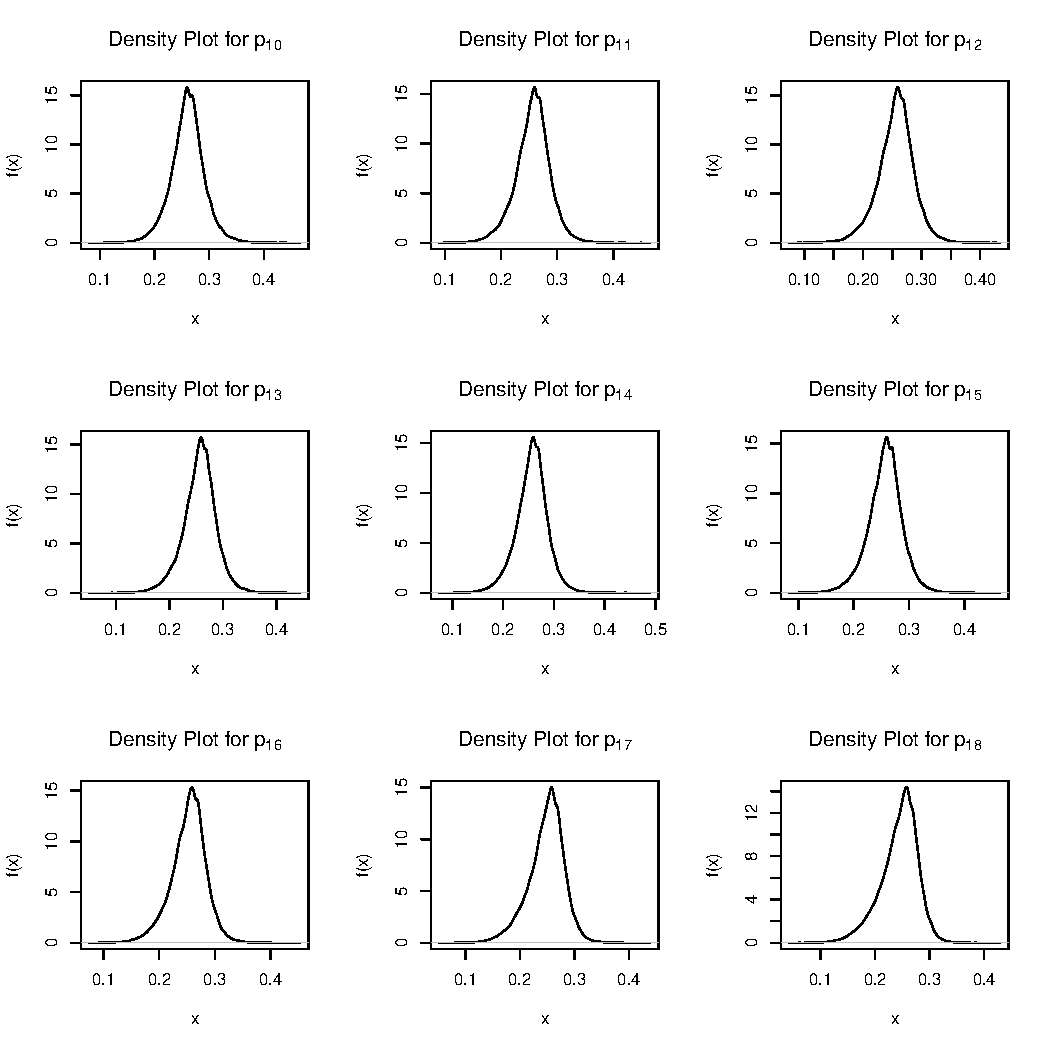
\includegraphics[scale=0.8]{pdensity2.pdf}
\end{center}
\caption{Posterior Density plots for $p_i, i = 10, ..., 18$} 
\label{dens2}
\end{figure}  
A comparison of the means under the model presented is shown in Table
\ref{tab1}. Its clear that the Efron-Morris is superior, but the James
Stein Estimator is worse than the Bayes Estimators we get from the simulations. 
\begin{table}[ht]
\centering
\textbf{Comparison of Estimates:}
\scalebox{0.75}{
\begin{tabular}{rlrrrr}
\hline
  \hline
 & Player & True Value & Stein & Efron-Morris & Posterior Means \\ 
  \hline
1 & Clemente,Roberto & 0.346 & 0.290 & 0.334 & 0.287 \\ 
  2 & Robinson,Frank & 0.298 & 0.286 & 0.313 & 0.283 \\ 
  3 & Howard,Frank & 0.276 & 0.282 & 0.292 & 0.279 \\ 
  4 & Johnstone,Jay & 0.222 & 0.277 & 0.277 & 0.276 \\ 
  5 & Berry,Ken & 0.273 & 0.273 & 0.273 & 0.272 \\ 
  6 & Spencer,Jim & 0.270 & 0.273 & 0.273 & 0.272 \\ 
  7 & Kessinger,Don & 0.265 & 0.268 & 0.268 & 0.268 \\ 
  8 & Alvarado,Luis & 0.210 & 0.264 & 0.264 & 0.265 \\ 
  9 & Santo,Ron & 0.269 & 0.259 & 0.259 & 0.260 \\ 
  10 & Swaboda,Ron & 0.230 & 0.259 & 0.259 & 0.261 \\ 
  11 & Petrocelli,Rico & 0.264 & 0.254 & 0.254 & 0.256 \\ 
  12 & Rodriguez,Ellie & 0.226 & 0.254 & 0.254 & 0.256 \\ 
  13 & Scott,George & 0.303 & 0.254 & 0.254 & 0.256 \\ 
  14 & Unser,Del & 0.264 & 0.254 & 0.254 & 0.256 \\ 
  15 & Williams,Billy & 0.330 & 0.254 & 0.254 & 0.256 \\ 
  16 & Campaneris,Bert & 0.285 & 0.249 & 0.249 & 0.252 \\ 
  17 & Munson,Thurman & 0.316 & 0.244 & 0.244 & 0.248 \\ 
  18 & Alvis,Max & 0.200 & 0.239 & 0.239 & 0.244 \\ 
   \hline
& Mean Squared Error & &0.0007392538&5.760222e-05 &  0.0005306359\\
   \hline
\hline
\end{tabular}
}
\caption{Table comparing the Stein,Efron-Morris and Bayes Estimates for $\chi^2_1$} 
\label{tab1}
\end{table}



The probability that the hitting average of player 2 is greater than
player 1 is $P(p_1<p_2)$. It can be estimated using:
\[
\hat{I} = \frac{1}{n} \sum_{i=1}^n I_{[{p}^i_1 <{p}^i_2]} =   0.46747.
\]

\pagebreak

\paragraph{2.} If we consider the following hierarchical Bayes model:
\[
X_i|\theta_i \sim \normd (\theta_i,1)
\]
\[
\theta_i| \mu, \tau^2 \sim \normd (\mu,\tau^2)
\]
\[
\mu \sim \normd(0,1000)
\]
\[
\tau^2 \sim \chi^2_5
\]
then, it seems like the $p_i$'s are shrinking less towards the mean. It is even
better than the Stein estimator as Table \ref{tab2} shows, however the Efron Morris estimator is
still clearly better, when compared to the real data. 
\begin{table}[ht]
\centering
\textbf{Comparison of Estimates:}
\scalebox{0.75}{
\begin{tabular}{rlrrrr}
  \hline
\hline
 & Player & True Value & Stein & Efron-Morris & Posterior Means \\ 
   \hline
1 & Clemente,Roberto & 0.346 & 0.290 & 0.334 & 0.328 \\ 
  2 & Robinson,Frank & 0.298 & 0.286 & 0.313 & 0.318 \\ 
  3 & Howard,Frank & 0.276 & 0.282 & 0.292 & 0.308 \\ 
  4 & Johnstone,Jay & 0.222 & 0.277 & 0.277 & 0.297 \\ 
  5 & Berry,Ken & 0.273 & 0.273 & 0.273 & 0.287 \\ 
  6 & Spencer,Jim & 0.270 & 0.273 & 0.273 & 0.287 \\ 
  7 & Kessinger,Don & 0.265 & 0.268 & 0.268 & 0.277 \\ 
  8 & Alvarado,Luis & 0.210 & 0.264 & 0.264 & 0.266 \\ 
  9 & Santo,Ron & 0.269 & 0.259 & 0.259 & 0.255 \\ 
  10 & Swaboda,Ron & 0.230 & 0.259 & 0.259 & 0.255 \\ 
  11 & Petrocelli,Rico & 0.264 & 0.254 & 0.254 & 0.245 \\ 
  12 & Rodriguez,Ellie & 0.226 & 0.254 & 0.254 & 0.244 \\ 
  13 & Scott,George & 0.303 & 0.254 & 0.254 & 0.244 \\ 
  14 & Unser,Del & 0.264 & 0.254 & 0.254 & 0.245 \\ 
  15 & Williams,Billy & 0.330 & 0.254 & 0.254 & 0.245 \\ 
  16 & Campaneris,Bert & 0.285 & 0.249 & 0.249 & 0.234 \\ 
  17 & Munson,Thurman & 0.316 & 0.244 & 0.244 & 0.222 \\ 
  18 & Alvis,Max & 0.200 & 0.239 & 0.239 & 0.211 \\ 
   \hline
& Mean Squared Error & &0.0007392538&5.760222e-05 & 0.0003418886\\
   \hline
\hline
\end{tabular}
}
\caption{Table comparing the Stein,Efron-Morris and Bayes Estimates for $\chi^2_5$} 
\label{tab2}
\end{table}
 
\end{document}